% Proposal for COMP8240 Assessment Task #1 (Project Proposal)
% Uses the ACL style files (acl.sty), as required by the assessment brief.
% Compile in Overleaf using the "ACL Rolling Review / ACL 2023+" template:
%   https://github.com/acl-org/acl-style-files
% Files required alongside this one: acl.sty, acl_natbib.bst, references.bib

\documentclass[11pt]{article}
\usepackage[]{acl}
\usepackage{times}
\usepackage{latexsym}
\usepackage{microtype}
\usepackage{graphicx}
\usepackage{booktabs}
\usepackage{amsmath}
\usepackage{amssymb}

\title{Project Proposal: Replicating and Extending \\ \textit{How Powerful are Graph Neural Networks?}}

\author{
  Sobhan Salarian \\
  Macquarie University \\
  COMP8240: Applications of Data Science \\
  \texttt{shaygan.sobhan79@gmail.com}
}

\begin{document}
\raggedbottom
\maketitle

\begin{abstract}
This proposal outlines a plan to replicate \citet{xu2019gin}, \textit{How Powerful are Graph Neural Networks?} (ICLR 2019), which develops a theoretical framework for the expressive power of Graph Neural Networks (GNNs) and introduces the Graph Isomorphism Network (GIN), a GNN architecture proven to be as powerful as the Weisfeiler-Lehman graph isomorphism test. We describe the paper's contributions for a general computer science audience, explain its evaluation methodology and benchmark datasets in detail, and justify the choice of this paper on grounds of venue quality, citation impact, and code/data accessibility. We confirm a preliminary feasibility check -- the official implementation has been downloaded and executed successfully on a sample dataset. Finally, we outline a plan to apply the method to new data: several existing but not-yet-tried datasets, and a new dataset we will construct by scraping actor-collaboration networks from The Movie Database (TMDb), mirroring the construction of the paper's own IMDB-BINARY and IMDB-MULTI benchmarks.
\end{abstract}

\section{Introduction}
Graph-structured data -- molecules, social networks, citation graphs -- is common across science and industry, and Graph Neural Networks (GNNs) have become the dominant tool for learning from it. Despite their empirical success, before \citet{xu2019gin} it was not well understood \emph{how expressive} GNNs actually are: which graphs a GNN can, in principle, ever learn to tell apart, regardless of how it is trained. This paper answers that question theoretically and uses the answer to design a maximally expressive GNN, the Graph Isomorphism Network (GIN).

This project will replicate the paper's empirical results on a subset of its benchmark datasets, and then test whether its central claim -- that GIN outperforms weaker GNN variants because it is more expressive -- continues to hold on new data that the method has never been applied to. This document is a proposal: it describes the paper, its evaluation methodology, our justification for choosing it, and our plan for sourcing and constructing new data. It does not report results; those will follow in the Update Presentation and Final Report.

\section{Description of the Paper}
\label{sec:description}

\subsection{Background: Message Passing on Graphs}
A GNN learns a vector representation (an \emph{embedding}) for each node in a graph, and then, for whole-graph tasks such as classification, combines all node embeddings into a single graph-level embedding. Node embeddings are learned through \emph{message passing}: in each round, every node gathers (\emph{aggregates}) the embeddings of its immediate neighbours, combines this aggregated information with its own current embedding, and produces an updated embedding. After several rounds, a node's embedding reflects information from an increasingly large neighbourhood around it. The final graph-level embedding is typically produced by \emph{pooling} (e.g., summing or averaging) all node embeddings together, and is then passed to a classifier.

Different GNN architectures -- Graph Convolutional Networks \citep[GCN;][]{kipf2017gcn}, GraphSAGE \citep{hamilton2017graphsage}, and others -- differ mainly in how they define the aggregation and combination steps. \citet{xu2019gin} ask a question that is orthogonal to any single architecture's empirical performance: given this general message-passing framework, what is the theoretical ceiling on what \emph{any} such architecture can distinguish?

\subsection{The Core Question: Expressive Power}
Two graphs are \emph{isomorphic} if one can be relabelled into the other -- they are structurally identical. A GNN that maps two non-isomorphic graphs to the same embedding has failed to distinguish them, no matter how well it is trained afterwards, because the representations are indistinguishable to any downstream classifier. \citet{xu2019gin} show that the aggregation function a GNN uses determines what it can and cannot distinguish. Specifically, they connect GNN expressiveness to the classical \emph{Weisfeiler-Lehman (WL) test} \citep{weisfeiler1968reduction}, a longstanding (non-learned) heuristic algorithm for graph isomorphism testing that also proceeds by iteratively aggregating neighbourhood information (see also its use as a graph kernel; \citealp{shervashidze2011wlkernel}).

The paper's central theoretical result is that the WL test is an \emph{upper bound} on what any message-passing GNN can distinguish: no GNN built purely from this neighbourhood-aggregation framework can be more powerful than the WL test. It then shows that popular aggregation choices used in practice -- mean-pooling (as in GCN) and max-pooling (which the paper shows approximates GraphSAGE) -- are \emph{strictly less} powerful than the WL test, because they can conflate structurally different neighbourhoods. A simple illustration is given in Figure~\ref{fig:multiset}: a node with two identical neighbour values and a node with four identical neighbour values have the same \emph{mean}, so a GNN using mean-aggregation cannot tell these two local structures apart, whereas a GNN using \emph{sum}-aggregation can, since the sums differ.

\begin{figure}[t]
\centering
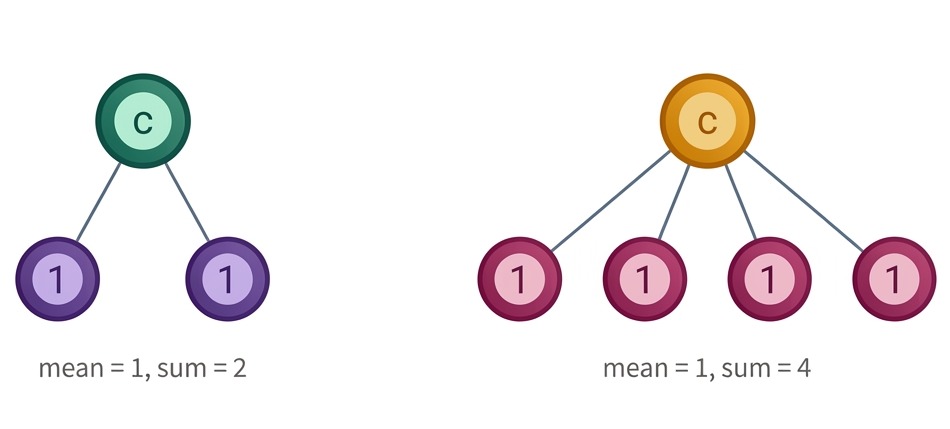
\includegraphics[width=\columnwidth]{figure1.png}
\caption{Illustrative example (after \citealp{xu2019gin}): two different neighbourhoods around a centre node \emph{c} that mean-aggregation maps to the same value, but sum-aggregation distinguishes.}
\label{fig:multiset}
\end{figure}

\subsection{The Graph Isomorphism Network (GIN)}
Building on this analysis, the paper proposes GIN, which uses \emph{sum}-aggregation followed by a multi-layer perceptron (MLP) to combine neighbourhood information. Concretely, node $v$'s representation at layer $k$ is updated as
\begin{equation}
\resizebox{0.85\linewidth}{!}{$h_v^{(k)} = \mathrm{MLP}^{(k)}\Big((1+\epsilon^{(k)}) h_v^{(k-1)} + \sum\limits_{u \in \mathcal{N}(v)} h_u^{(k-1)}\Big)$}
\label{eq:gin}
\end{equation}
where $\mathcal{N}(v)$ is $v$'s neighbour set and $\epsilon^{(k)}$ weights a node's own representation against its neighbours' sum. The authors prove that this design is exactly as powerful as the WL test -- the maximum achievable within the message-passing framework. GIN is therefore not proposed as an incrementally better heuristic, but as a provably optimal instance of its model class.

\subsection{Contributions Summary}
The paper's contributions are: (1) a theoretical framework relating GNN expressiveness to the WL test; (2) proof that GIN achieves the maximum expressiveness possible for message-passing GNNs; (3) a formal explanation of why widely used variants (GCN, GraphSAGE) are strictly less expressive; and (4) empirical validation across nine graph-classification benchmarks, where GIN matches or exceeds both the WL subtree kernel and prior GNN architectures.

\section{Explanation of Evaluation}
\label{sec:evaluation}

\subsection{Task and Protocol}
The paper evaluates on \emph{graph classification}: each input is an entire graph (e.g., a molecule or a social ego-network), and the model must predict one of $k$ class labels for it (e.g., whether a molecule is mutagenic, or which genre a social network was drawn from). Because several benchmark datasets are small (the smallest has under 200 graphs), the paper does not use a single fixed train/test split; instead it uses \textbf{10-fold cross-validation}: the dataset is partitioned into 10 folds, the model is trained on 9 and evaluated on the held-out fold, this is rotated across all 10 folds, and the reported result is the mean test accuracy $\pm$ one standard deviation across folds.

A subtlety not spelled out in the paper's main text, which we will confirm directly from the released implementation before replicating: because test accuracy fluctuates across training epochs, a rule is needed to select \emph{which} epoch's accuracy to report. We will verify from the official code which of the plausible conventions is used -- e.g., averaging the 10 folds' per-epoch accuracy curves and reporting the mean $\pm$ std at whichever epoch that averaged curve peaks -- since reporting each fold's own best epoch independently would optimistically bias the result.

Table~\ref{tab:worked} illustrates why this distinction matters, with a small toy example (3 folds, 4 epochs). The correct rule averages the three folds \emph{per epoch}, finds that epoch 30 has the highest such average (0.753), and reports the mean $\pm$ std of the three folds' individual accuracies \emph{at epoch 30} (0.753 $\pm$ 0.017). A naive but biased alternative would instead take each fold's own best epoch independently -- Fold 1 peaks at epoch 20 (0.75), Fold 2 at epoch 40 (0.78), Fold 3 at epoch 30 (0.76) -- and average those together to get 0.763, silently inflating the reported score above what any single, fixed stopping point would actually have achieved.

\begin{table}[t]
\centering
\small
\begin{tabular}{lcccc}
\toprule
Epoch & Fold 1 & Fold 2 & Fold 3 & Average \\
\midrule
10 & 0.70 & 0.68 & 0.72 & 0.700 \\
20 & 0.75 & 0.74 & 0.71 & 0.733 \\
\textbf{30} & \textbf{0.73} & \textbf{0.77} & \textbf{0.76} & \textbf{0.753} \\
40 & 0.72 & 0.78 & 0.73 & 0.743 \\
\bottomrule
\end{tabular}
\caption{Toy illustration of the model-selection rule (invented numbers, for exposition only).}
\label{tab:worked}
\end{table}

\subsection{Baselines}
The paper compares GIN against: the WL subtree kernel \citep{shervashidze2011wlkernel}, a non-learned graph kernel method; several earlier graph kernel and CNN-on-graph methods (DCNN, PatchySAN, DGCNN); and, most relevantly for this project, weaker GNN aggregation variants -- including a \textbf{max-1-layer} configuration that the paper states corresponds to GraphSAGE \citep{hamilton2017graphsage} up to minor architectural differences, and mean-aggregation variants corresponding to GCN-style models. This is useful for our project because it means a GraphSAGE-style comparison point can potentially be obtained from the same, already-verified codebase, by changing aggregation/combination settings rather than integrating a second, independent implementation -- reducing engineering risk if we choose to include this comparison.

\subsection{Datasets Used in the Paper}
The paper evaluates on nine standard graph-classification benchmarks: four bioinformatics datasets with categorical node features (MUTAG, PTC, NCI1, PROTEINS), and five social-network datasets with no node features, where classification must rely on graph structure alone (COLLAB, IMDB-BINARY, IMDB-MULTI, REDDIT-BINARY, REDDIT-MULTI5K). Table~\ref{tab:datasets} gives statistics for all nine, taken directly from the paper.

\begin{table}[t]
\centering
\resizebox{\columnwidth}{!}{%
\begin{tabular}{lccc}
\toprule
Dataset & \#Graphs & \#Classes & Avg.\ \#Nodes \\
\midrule
MUTAG & 188 & 2 & 17.9 \\
PTC & 344 & 2 & 25.5 \\
NCI1 & 4110 & 2 & 29.8 \\
PROTEINS & 1113 & 2 & 39.1 \\
COLLAB & 5000 & 3 & 74.5 \\
IMDB-BINARY & 1000 & 2 & 19.8 \\
IMDB-MULTI & 1500 & 3 & 13.0 \\
REDDIT-BINARY & 2000 & 2 & 429.6 \\
REDDIT-MULTI5K & 5000 & 5 & 508.5 \\
\bottomrule
\end{tabular}}
\caption{All nine benchmark datasets used in \citet{xu2019gin}; statistics as reported in the paper's own dataset table.}
\label{tab:datasets}
\end{table}

The bioinformatics/social-network split matters for feature engineering: the four bioinformatics datasets use each dataset's categorical node labels as input, whereas the five social-network datasets have no node attributes at all, so the paper falls back to structural proxies (node degree, or a constant feature for the two REDDIT datasets) to force the model to rely purely on graph topology. Notably, the paper reports it could not run its max-pooling (GraphSAGE-style) variant on REDDIT-BINARY, REDDIT-MULTI5K, or COLLAB due to GPU memory constraints -- worth keeping in mind if we later extend our own GraphSAGE-style comparison beyond IMDB-BINARY/IMDB-MULTI.

We plan to focus our replication on \textbf{IMDB-BINARY} and \textbf{IMDB-MULTI}, since these are the two datasets for which we intend to build a matching new-data construction (Section~\ref{sec:newdata2}), allowing a direct, apples-to-apples comparison between replicated original results and results on new data. Both were originally released by \citet{yanardag2015deep} (\textit{Deep Graph Kernels}), not by \citet{xu2019gin}, who reuse them as a benchmark; we cite the original release paper as the authoritative description of how they were built. In both datasets, a graph represents one actor's ego-network of collaborators: nodes are actors, an edge connects two actors who co-starred in a film, and the graph label is the genre of that ego-network's associated film community (IMDB-BINARY: Action vs. Romance; IMDB-MULTI: Comedy vs. Romance vs. Sci-Fi). Neither dataset provides node attributes, so \citet{xu2019gin} use each node's degree as its only input feature -- a detail that matters for interpreting results on any new data built the same way, since the model has no richer signal to fall back on.

\subsection{Towards an LLM-as-Judge Evaluation}
Accuracy against a hard ground-truth genre label is well suited to automatic scoring and does not, on its own, call for an LLM judge. However, an LLM-as-judge could plausibly add value as a complementary, qualitative check: for graphs the model misclassifies, we could describe the ego-network (e.g., its cast list) in text and ask an LLM whether the assigned genre label is itself plausible, as a sanity check on label quality in any dataset we construct ourselves. As this topic will be covered in detail later in the unit (Week 7 onward), we do not commit to a specific method here; this is an initial direction we intend to refine once appropriate methodology has been introduced.

\section{Justification for Paper Choice}
\label{sec:justification}

\subsection{Research Quality Indicators}
We justify choosing this paper on several independent grounds:
\begin{itemize}
    \item \textbf{Venue quality:} the paper appeared at ICLR, ranked A* by the CORE conference ranking, a top-tier venue for representation learning.
    \item \textbf{Citation impact:} the paper is one of the most cited works in graph representation learning, widely regarded as a foundational theoretical result for the field; we will report the current citation count (from Google Scholar or Semantic Scholar) at the time of the Final Report, since this figure changes continually.
    \item \textbf{Community adoption:} the official code repository has attracted substantial independent use (over one thousand GitHub stars and over two hundred forks at the time of writing), indicating the implementation is actively relied upon rather than an abandoned research artifact.
    \item \textbf{Theoretical grounding:} unlike papers that report a new architecture's empirical performance alone, this paper proves a tight bound on expressiveness, giving a stronger basis for understanding \emph{why} an empirical result should be expected to hold or fail on new data -- directly useful for the investigative aim of this project.
\end{itemize}

\subsection{Feasibility}
As a basic feasibility check, we have downloaded the official implementation and executed it successfully end-to-end on a sample dataset (MUTAG) in a local environment, confirming that the code, its dependencies, and the bundled data all work together without modification. Beyond this preliminary check, we note the following in support of feasibility for the full project:
\begin{itemize}
    \item \textbf{Code accessibility:} the official implementation is public and uses a standard, actively maintained deep learning stack (PyTorch), with no closed dependencies.
    \item \textbf{Data availability:} all nine benchmark datasets are bundled directly with the official repository, removing the risk of relying on an external dataset host that may become unavailable.
    \item \textbf{Suitability for new-data extension:} because the task is graph classification with a self-contained cross-validation protocol (rather than, e.g., transductive node classification on one fixed graph), it is comparatively straightforward to point the same pipeline at a newly constructed dataset without modifying the model or training code.
    \item \textbf{Compute resources:} the paper's protocol (350 epochs $\times$ 10 folds per dataset) exceeds what a laptop CPU can comfortably run within the project timeline. Our primary planned resource is a free-tier Google Colab GPU instance, which the official code already supports unmodified (it auto-detects CUDA); as a fallback if Colab's usage limits become a bottleneck, we also have SSH access to a university lab GPU server.
\end{itemize}
We are not reporting technical results at this stage, in line with the scope of this assessment; a fuller account of replication progress will be given in the Update Presentation.

\section{New Data}
\label{sec:newdata}

\subsection{Existing Datasets Not Yet Applied to This Method}
\label{sec:newdata1}
We have identified five candidate existing datasets to which the GIN method has not, to our knowledge, been directly applied in the original paper, and assessed the feasibility of each:

\begin{enumerate}
    \item \textbf{Additional TU Dataset benchmarks} (e.g., ENZYMES, DD), from the same benchmark collection as the paper's own nine datasets. Feasibility is very high, since these already ship in the exact input format the official code expects; the main limitation is that they are close in kind to the original benchmark suite, so they add less novelty than the other options below.
    \item \textbf{Open Graph Benchmark (OGB) graph-classification datasets} \citep{hu2020ogb}, e.g., ogbg-molhiv. Feasibility is high -- OGB is maintained by an overlapping author group and provides PyTorch-native loaders -- but would require writing a small adapter to convert into the TU-style text format the official GIN code reads.
    \item \textbf{AIDS, hosted on the HuggingFace Datasets Hub} under the \texttt{graphs-datasets} organisation -- a molecular graph-classification dataset of antiviral screening compounds ($\sim$2000 graphs). Feasibility is high (a ready-made HuggingFace loader exists), though it needs a small script to convert into the plain-text TU format the official GIN code reads, similar in effort to the OGB candidate above. It is itself part of the wider TU benchmark family (like candidate 1), so its main distinguishing value here is tooling convenience rather than a genuinely different data domain.
    \item \textbf{A molecule/chemistry dataset from Kaggle} (e.g., a Tox21- or QM9-derived toxicity or property-classification subset). Plausible in principle, but requires per-dataset verification of labelling quality and licensing terms before committing.
    \item \textbf{A co-authorship network dataset built from the OpenAlex API}, structurally analogous to the paper's COLLAB benchmark (graphs of collaborators). This is the most conceptually novel option but also the most engineering-heavy, since we would need to define graph boundaries (e.g., one graph per author's co-author ego-network) ourselves rather than using an existing packaged dataset -- it is, in effect, a bridge toward the newly-constructed-data category below.
\end{enumerate}

\subsection{Newly Constructed Data}
\label{sec:newdata2}
In addition to existing datasets, we plan to construct a new dataset that mirrors the construction recipe of the paper's own IMDB-BINARY and IMDB-MULTI benchmarks, but built from more recent source data. Figure~\ref{fig:pipeline} summarises this plan: the same four-step recipe (movies $\rightarrow$ cast $\rightarrow$ collaboration graph $\rightarrow$ genre label) applied to a new source, feeding into the identical, unmodified GIN pipeline used for the original data.

\begin{figure}[t]
\centering
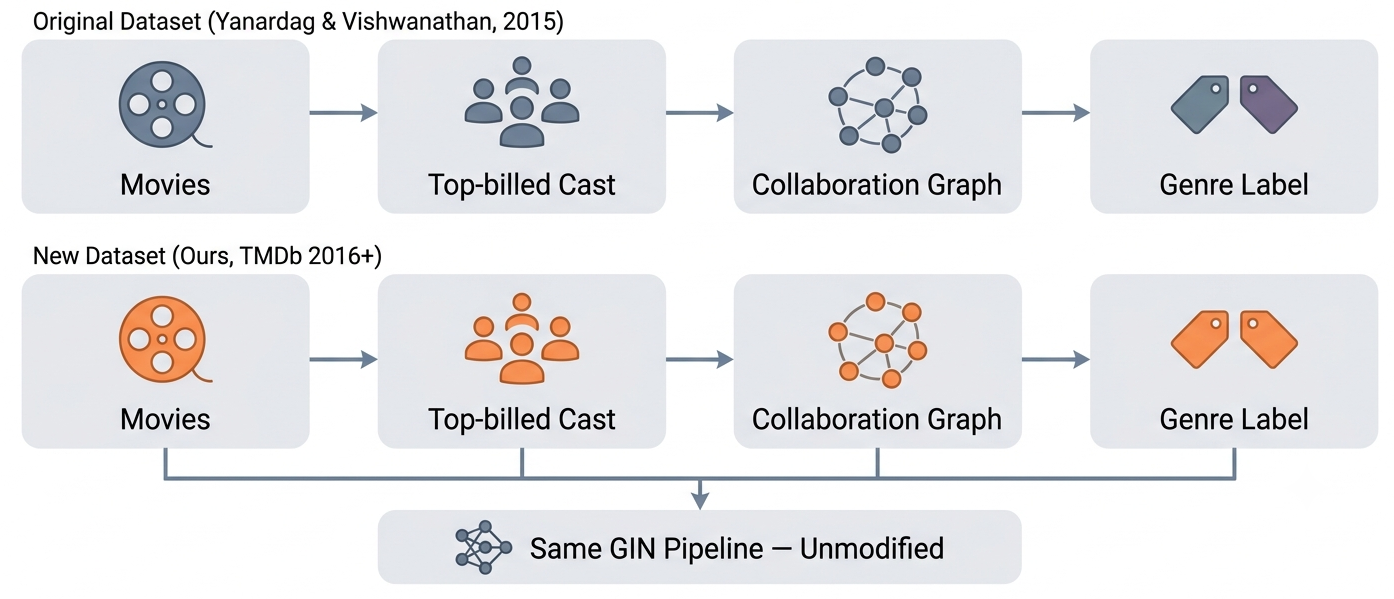
\includegraphics[width=\columnwidth]{pipeline.png}
\caption{Planned construction pipeline for the new dataset, mirroring the original IMDB-BINARY/IMDB-MULTI recipe \citep{yanardag2015deep} on newer source data, so that it feeds into the same, unmodified GIN pipeline.}
\label{fig:pipeline}
\end{figure}

\textbf{Source.} We will use The Movie Database (TMDb) API \citep{tmdb}, which provides a free developer key and programmatic access to film metadata and cast listings. Any use will include the attribution TMDb's terms require: \textit{``This product uses the TMDb API but is not endorsed or certified by TMDb.''}

\textbf{Construction plan.} Following the same recipe as \citet{yanardag2015deep}, we plan to: (i) restrict to films released from 2016 onward, to avoid any overlap with the original dataset's 2015 construction date; (ii) keep only films whose genre metadata contains exactly one of our target genres, to avoid ambiguous multi-genre labels; (iii) take each film's top-billed cast as the node set for that film's graph; and (iv) connect two actors with an edge if they have co-appeared in any sampled film of that genre, producing an actor-collaboration ego-network structure analogous to the original construction, rather than one isolated clique per film. We will target a similar overall scale to the originals (on the order of 1{,}000 graphs for the binary genre task and 1{,}500 for the three-way genre task), and will write the output directly in the input format the official GIN code expects, so that no changes to the model or training pipeline are needed to run it on this new data once built.

\textbf{Labels and human judgement.} Genre labels for this dataset come directly from TMDb's existing metadata rather than requiring new human annotation, since genre classification is part of the platform's own curated data. If we pursue the OpenAlex-based co-authorship dataset described above as a second new dataset, we similarly expect to draw ground-truth structure directly from the source platform rather than requiring a separate annotation effort; as this course topic is addressed later in the unit, a more detailed annotation methodology will be developed once introduced.

\section{Planned Work}
\label{sec:plan}
Building on the feasibility check already completed, our plan for the remainder of the project is to: (1) replicate the paper's reported results on IMDB-BINARY and IMDB-MULTI using the official implementation and the evaluation protocol described in Section~\ref{sec:evaluation}; (2) construct the new TMDb-based dataset described in Section~\ref{sec:newdata2} and apply the identical, unmodified pipeline to it, to test whether the paper's central claim continues to hold on data the method has not previously seen; (3) time permitting, extend the comparison to a GraphSAGE-style baseline using the architecture variant the paper itself defines (Section~\ref{sec:evaluation}), to see whether any gap between GIN and less expressive GNNs behaves consistently between the original and new data; and (4) investigate qualitatively where and why the method succeeds or fails, including on individual misclassified examples. Detailed results for these steps will be presented in the Update Presentation and Final Report, not in this proposal.

\section{Conclusion}
This proposal has described \citet{xu2019gin}'s theoretical contribution and empirical evaluation, justified our choice of this paper for replication, and outlined a two-part plan for new data: exploring existing datasets the method has not yet been applied to, and constructing a new actor-collaboration dataset via the TMDb API that mirrors the original benchmark's own construction. Having confirmed the official implementation runs successfully in our environment, we consider this project feasible and will proceed to full replication and new-data evaluation.

\bibliography{references}

\end{document}
